\chapter{Causal Graph}\label{ch:causal-graph}
In this chapter, we want to provide a methodology to generate a \ac{WDCG} from \ac{CEP}s, as well as for the flight logs dataset.
The nodes in the \ac{WDCG} consist of the phrases, and the edges represent a causal relation between two nodes.
The edges also contain a numerical weight that represents the occurrence of such relationships in the source.
We also provide a tool that visualizes such \ac{WDCG} and allows to interactively examine the graph.


\section{Graph From Cause-Effect Pairs}\label{sec:graph-from-cause-effect-pairs}
\begin{figure}
    \begin{center}
        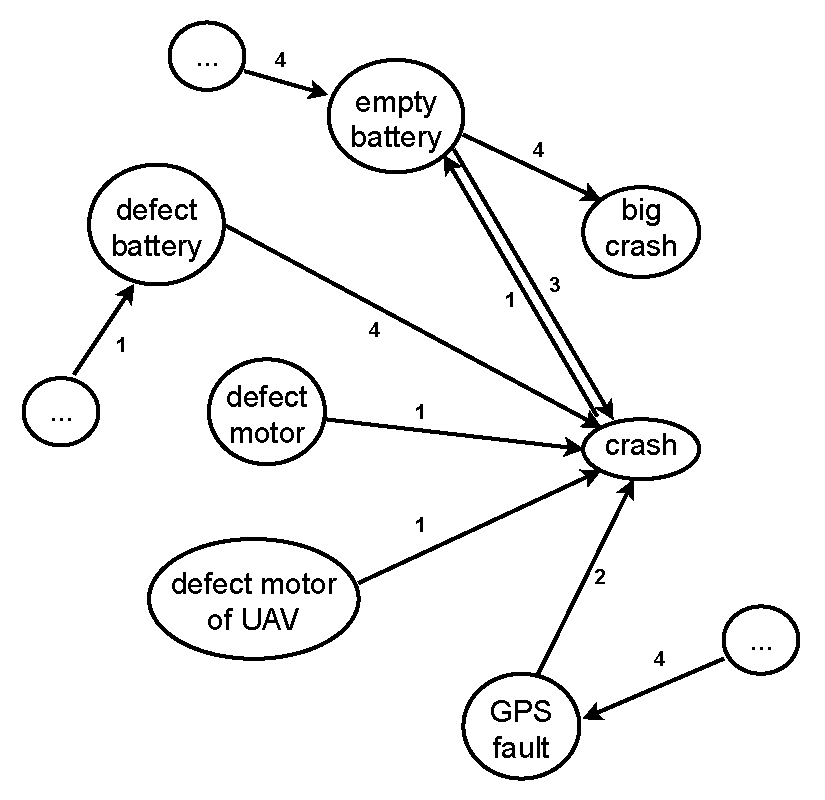
\includegraphics[scale=.6]{figures/causal_graph/causal_graph}
        \caption{Weighted Directed Causal Graph}\label{fig:causal-graph}
    \end{center}
\end{figure}
The previous pipeline step produced multiple \ac{CEP}s.
However, different users may use different words to mean the same thing.
Thus, one user could say \qq{GPS fault causes crash} another would say \qq{GPS error causes crash} so that the cause would be \qq{GPS fault} and \qq{GPS error}.
We used the idea from \cite{Hassanzadeh19} to create a synonym dictionary to replace similar words with a matching synonym in the dictionary
We first created a dictionary that counts all the unique tokens that appear in the \ac{CEP}s, which we sorted in descending order based on the occurrence.
The dictionary indicates the rank of each word in the corpus.
The first element of the dictionary represents the word that the users mostly use.
We then replaced each token of the \ac{CEP}.
To do so, we first used the wordnet corpus to find a list of synonyms for the tokens.
then loop through the sorted dictionaries from high to low occurrence and search for a matching synonym.
Such a hit represents either the same token or a synonym used more frequently by the domain experts.
If we hit such a synonym, we replace the token in the phrase with the synonym.
By following this approach for all phrases in the \ac{CEP}s, we produce a generalized representation of the \ac{CEP}s.
To build the \ac{WDCG} we are merging the same \ac{CEP}s into one \ac{CEP} with a weight attribute that represents the occurrence.
The \ac{CEP} with the weight describes two nodes in the graph, where the cause node has a directed weighted edge to the effect node
We build the \ac{WDCG} by merging the same nodes.
In \autoref{fig:causal-graph} we can see the resulting graph with some additional nodes and edges for the sentence \qq{A empty and defect battery, GPS fault or defect motor of UAV causes a crash}.


\section{Graph From Flight Logs Dataset}\label{sec:graph-from-flight-logs-dataset}
Unfortunately, there is no ground truth graph that we could validate our causal graph.
This section aims to provide the necessary steps to transform the provided flight logs dataset into a \ac{WDCG}.
We will use the resulting graphs in the \autoref{ch:evaluation-methods} module to evaluate the causal graph from the domain-experts with this graph.

\subsection{Flight Logs Dataset}\label{subsec:flight-logs-dataset}
\begin{table}
    \begin{center}
        \label{fig:verb-list}
        \begin{tabular}{||c c||}
            \hline
            ID & DICT \\ [0.5ex]
            \hline\hline
            16 & ekf check        \\
            \hline
            9  & failsafe fence   \\
            \hline
            9  & failsafe fence   \\
            \hline
            9  & failsafe fence   \\
            \hline
            16 & ekf check        \\
            \hline
            17 & failsafe ekfinav \\
            \hline
            16 & ekf check \\ [1ex]
            \hline
        \end{tabular}
    \end{center}
    \caption{\label{tab:flight-log-example-error-table}Flight log example error table}
\end{table}
The flight logs dataset contains thousands of flight logs.
Each flight log contains multiple time series tables, which represent a specific component in the UAV system, which logs the state of the attributes of such component by time.
For example the table \qq{EKF2} represents the \qq{EKF2 Estimation System} with different states such as \qq{attitude},  \qq{velocity'} or  \qq{position} as well as a \qq{timestamp}.
For the scope of the thesis, we will only consider the \qq{EV} and \qq{ERR} tables, which represent the  \qq{Event Subsystem} and the \qq{Error Subsystem}.
In \autoref{tab:flight-log-example-error-table} we can see such a table for the \qq{Error Subsystem}.
The origin table only consists of the ID column.
The DICT column represents the textual representation of the ID. ArduPilot provides a dictionary that maps these IDs into text, which can be found on GitHub \footnote{\url{https://github.com/ArduPilot/ardupilot/blob/master/libraries/AP\_Logger/AP\_Logger.h\#L94}}.
For example, the ID with the value \qq{17} represents \qq{FAILSAFE\_EKFINAV}.
To compare such a label, we decided to split it and used the lowercase representation of the words.
Thus, we would use \qq{failsafe ekfinav} instead of \qq{FAILSAFE\_EKFINAV} as the label.

\subsection{Transforming Into Causal Graph}\label{subsec:transforming-into-causal-graph}
To generate a causal graph from the flight logs data, we applied five steps:
\begin{enumerate}
    \item Create causality chain: We transform the time series tables (\qq{EV} and \qq{ERR}) of the flight logs into a chain of IDs, which is created in the time direction.
    Thus, in our example \autoref{tab:flight-log-example-error-table} we would generate the following chain \qq{16=>9=>9=>. . . =>9=>16=>17=>16}.
    This chain represents the different states of the subsystem in chronological order.
    \item Drop duplicate neighbors: We can see that such chain many of the same links can occur in succession because for these timestamps, the state did not change.
    Thus, we decided to drop such duplicates because they did not add information.
    The chain from the previous step would be processed to the chain \qq{16=>9=>16=>17=>16}.
    \item To structure the chain into a list of \ac{CEP}s, we extracted for each chain item the direct successor.
    Thus, we would extract \qq{16=>9}, \qq{9=>16}, \qq{16=>17}, \qq{17=>16} from the previous chain as \ac{CEP}s.
    This is our assumption, and we are aware that it is not correct in many cases.
    We do this to illustrate how validation could be done if we had ground truth graphs.
    By following steps 1 to 3 for each flight log, we can create a new dataset containing \ac{CEP}s.
    \item Reduce the pairs to a graph: We used the same approach from \autoref{sec:graph-from-cause-effect-pairs} to build a \ac{WDCG} from \ac{CEP}s.
    \item Convert the ids to text: Finally, we translate the numerical ids into textual phrases by using the ArduPilot dictionary.
\end{enumerate}


\section{Data Visualisation}\label{sec:datavisualisation}
To explore the causal graph, we built a visualization tool based on NetworkX\footnote{\url{https://networkx.org/}}, Plotly\footnote{\url{https://plotly.com/}}, and Dash\footnote{\url{https://plotly.com/dash/}}.
NetworkX is a python package for the creation and manipulation, and study of the structure of complex networks, like our causal graph.
We use this package to calculate the position of the nodes of the graph by using a Fruchterman-Reingold force-directed algorithm.
The algorithm holds nodes with treating edges close while treating nodes as repelling objects.
To visualize the graph, we use Plotly, which is an open-source graphing library that allows us to create interactive graphs by using different types of plots.
However, the Plotly library does not natively have an interface to build a directed graph.
To overcome this, we used a scatter plot, where the dots represent the nodes of the graph.
We decided not to draw edges in the default mode because such a graph can potentially have thousands of nodes and edges, which leads to the fact that the edges are not recognizable.
We used color scales to indicate nodes with high connectivity, which is useful to discover the graph.
Fortunate, Plotly allows us to interact with the graph, which is especially useful when dealing with a high amount of nodes.
To get information on the current node, we added a hover functionality that displays the name of the node as well as the name of the predecessors and successors of the node.
To discover the structure in a visual way, we can click a node, which draws all the edges as arrows that are related to the node.
We also added annotations that show the name of these nodes.
We used Dash to create an interactive web application, which runs the Plotly graph in the web browser.
